\section{Additional Implementation Details} % (fold)
\label{sec:positioning}

In the \ida{PNAI} reimplementation there are some details worthy of further discussion.
In this section the managing of devices in the desktop is explained.
Before there were always three devices in static positions, but now the system should be prepared to having an undefined number of devices.

\subsection{Positioning Devices} % (fold)
\label{sub:algorithm}

The first time that the user visits the page in a new browser, the system has to place the devices in the screen.
Since the number and type of devices -- therefore its size -- are different for each user, an algorithm must be calculated to placed the devices in the available space.
There are some restrictions that the algorithm have to comply with:

\begin{itemize}
  \item There is an undetermined number of elements to place.
  \item For the sake of simplicity, the elements and the canvas are rectangular.
  \item Every element, including the canvas, has a different size.
  \item The elements have to be placed in the most comfortable way possible for the user, ideally using all the available space.
\end{itemize}

The solution to the above problem is known as a variant of 2-D rectangle packing and it is, regrettably, NP-hard.
At this point, it is clear that we need a simplification.
Furthermore, the original problem also presents a big issue, as it does not address an important constraint: the possibility of resizing the elements to fit the canvas.

A simplified algorithm is proposed and implemented, relaxing some terms while obtaining acceptable results.
The important concepts are:

\begin{itemize}
  \item The main goal is to draw a virtual grid of M$\times$N cells (like a table).
  Every cell can be a position for a device.
  \item Indeed, we are going to calculate the smallest grid of M$\times$N cells in which the devices can be placed.
  \item Finally, we are going to resize the elements to fit within that cell, giving that every cell has the same size.

\end{itemize}

To obtain the squared grid for N elements, we simply have to calculate the ceiling of the squared root of N as seen in eq.~\eqref{gridx}.

\begin{equation}
  Grid_{x} = \lceil\sqrt{N}\rceil \label{gridx}
\end{equation}

This formula synthesizes the idea that, given a certain number of elements N:

\begin{itemize}
  \item If N is a square number (that is, it exists an integer $x$ that fulfills $x^2 = N$), then you could fit a whole grid of $x\times{}x$ with N elements.
  \item Otherwise, this integer N must be between the square of two consecutive integers, that we are going to call $x$ and $x+1$.
  That is, $x^2 < N$ and $(x+1)^2 > N$.
  In visual words, that means that a grid of size $x$ cannot hold that number of elements, and a grid of size $x+1$ can hold that number of elements but there will be empty \emph{cells}.
  \item In that case, we choose the grid of size $x+1$, this way we want to apply the ceiling function to the squared root to obtain the next following integer.
\end{itemize}

Figure~\vref{fig:algorithm-boxes} shows consecutive examples using from one element to thirteen elements, so that we can appreciate what all of this means.
Without looking very hard at the examples, we can guess an improvement without making the calculation severely complicate.

\begin{figure}[htbp]
  \centering
  \subfigure[1 element]{
    \label{fig:algorithm-boxes-1}
    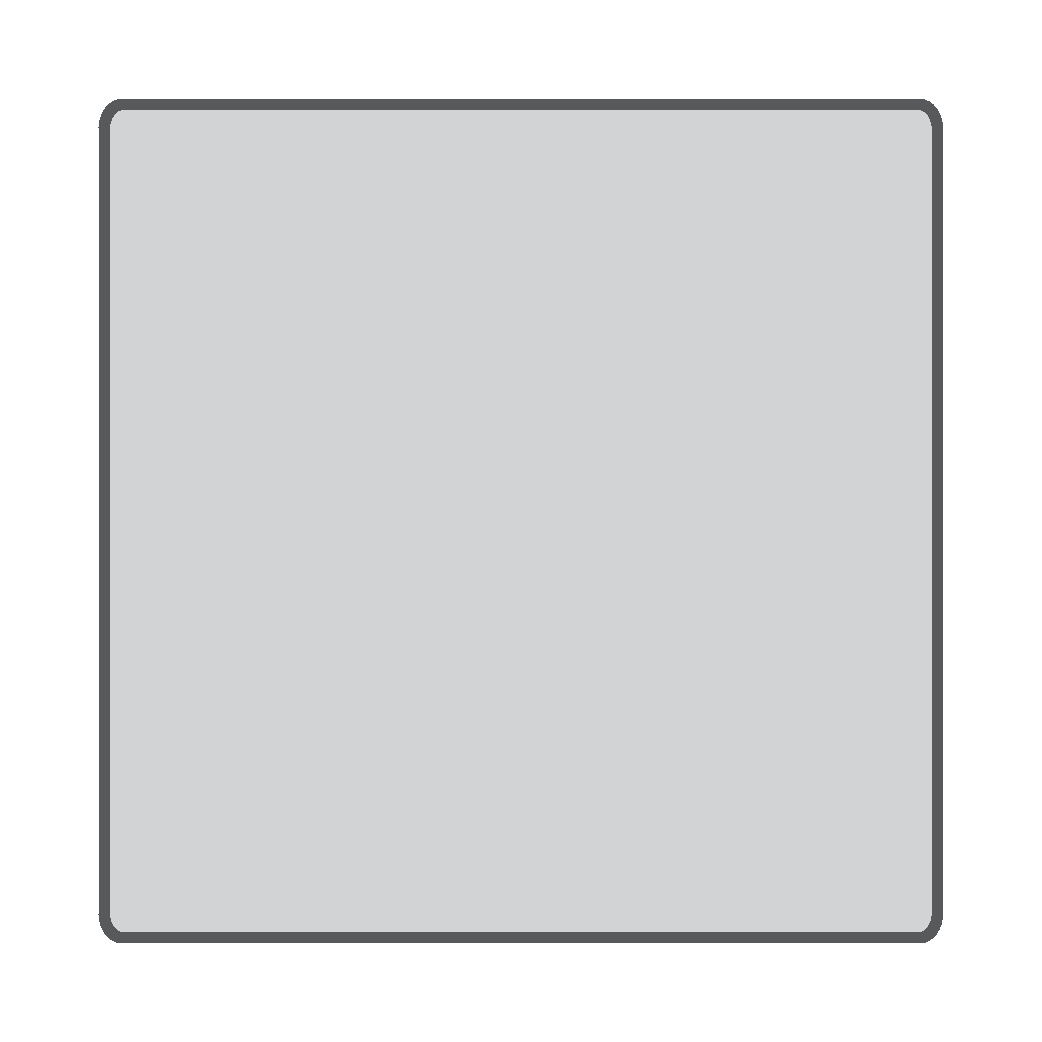
\includegraphics[width=0.3\textwidth]{algorithm-boxes-1}
  }
  \subfigure[2 elements]{
    \label{fig:algorithm-boxes-2}
    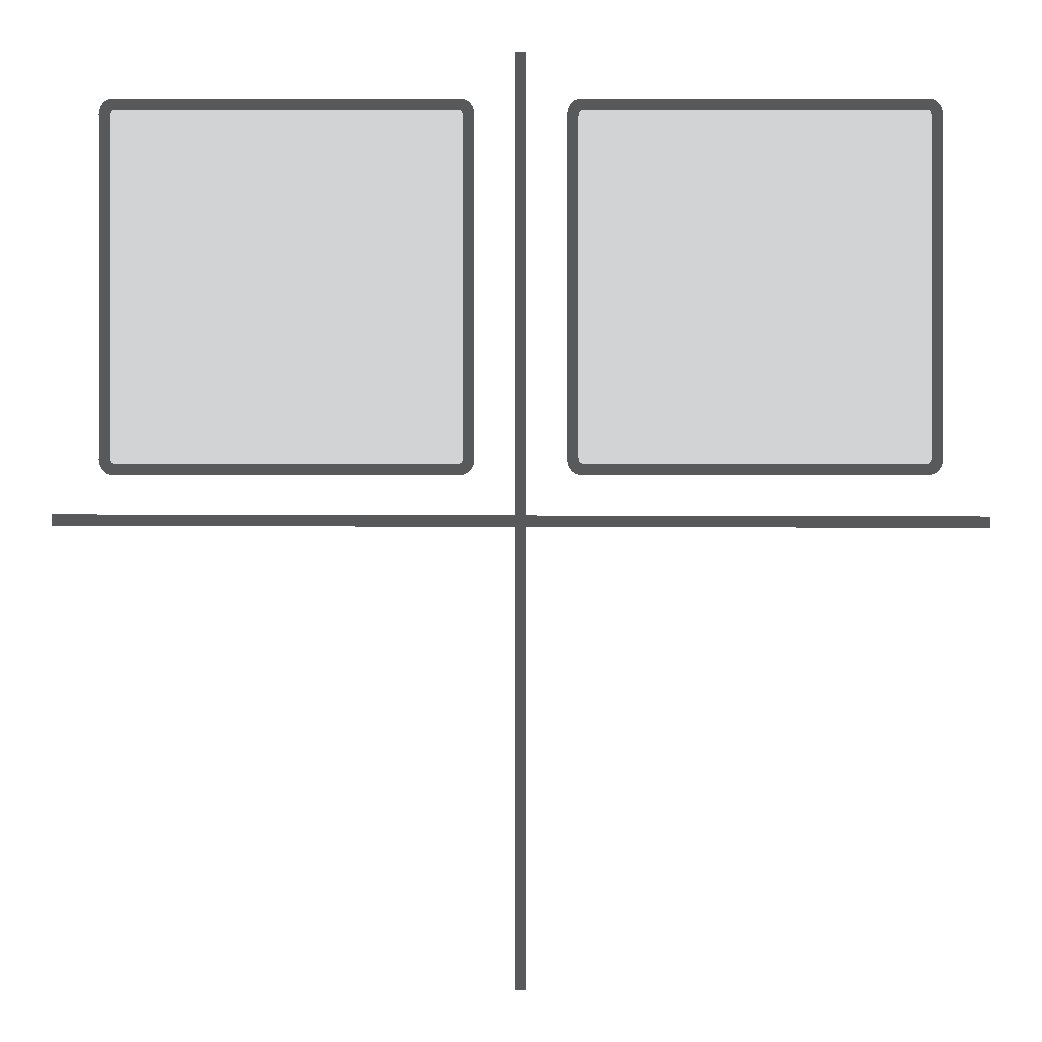
\includegraphics[width=0.3\textwidth]{algorithm-boxes-2}
  }
  \subfigure[3 elements]{
    \label{fig:algorithm-boxes-3}
    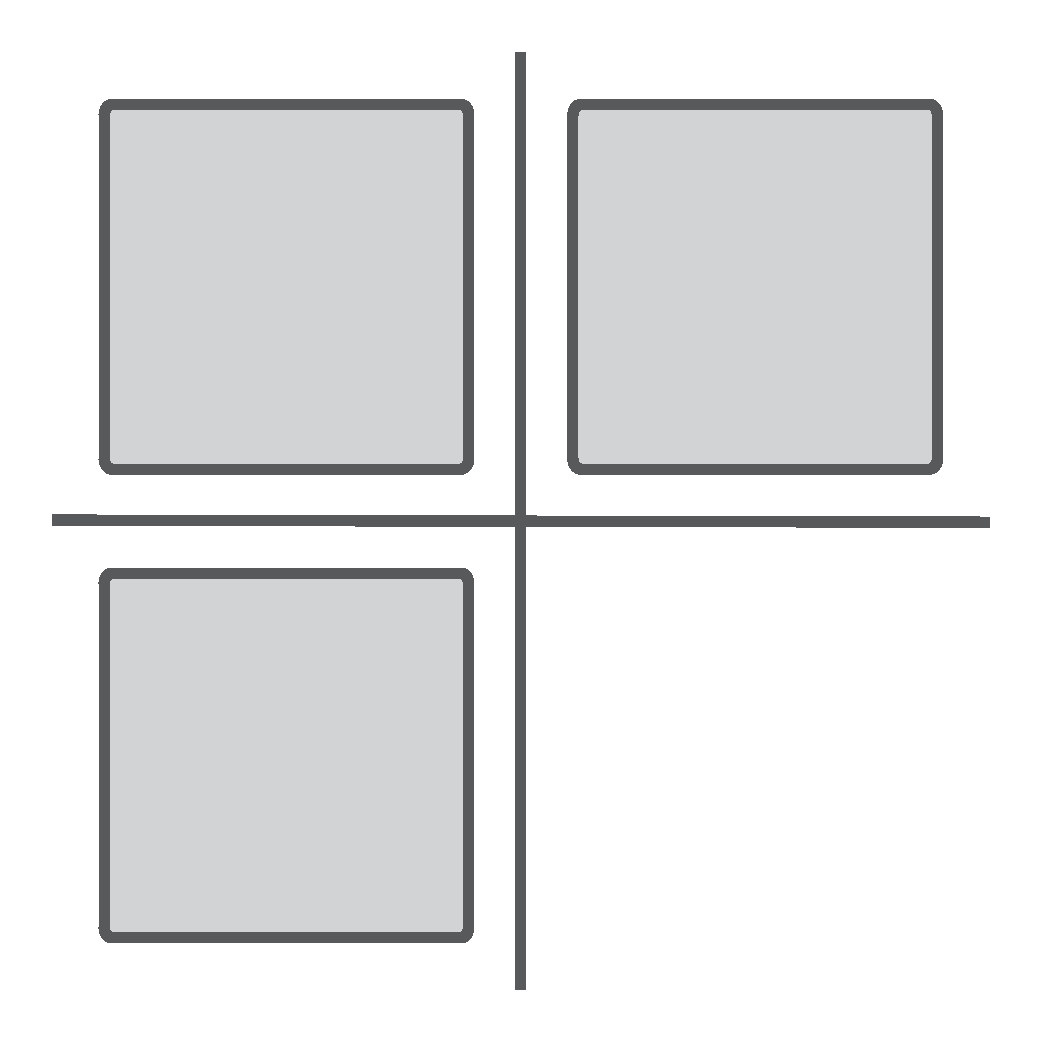
\includegraphics[width=0.3\textwidth]{algorithm-boxes-3}
  }
  \subfigure[4 elements]{
    \label{fig:algorithm-boxes-4}
    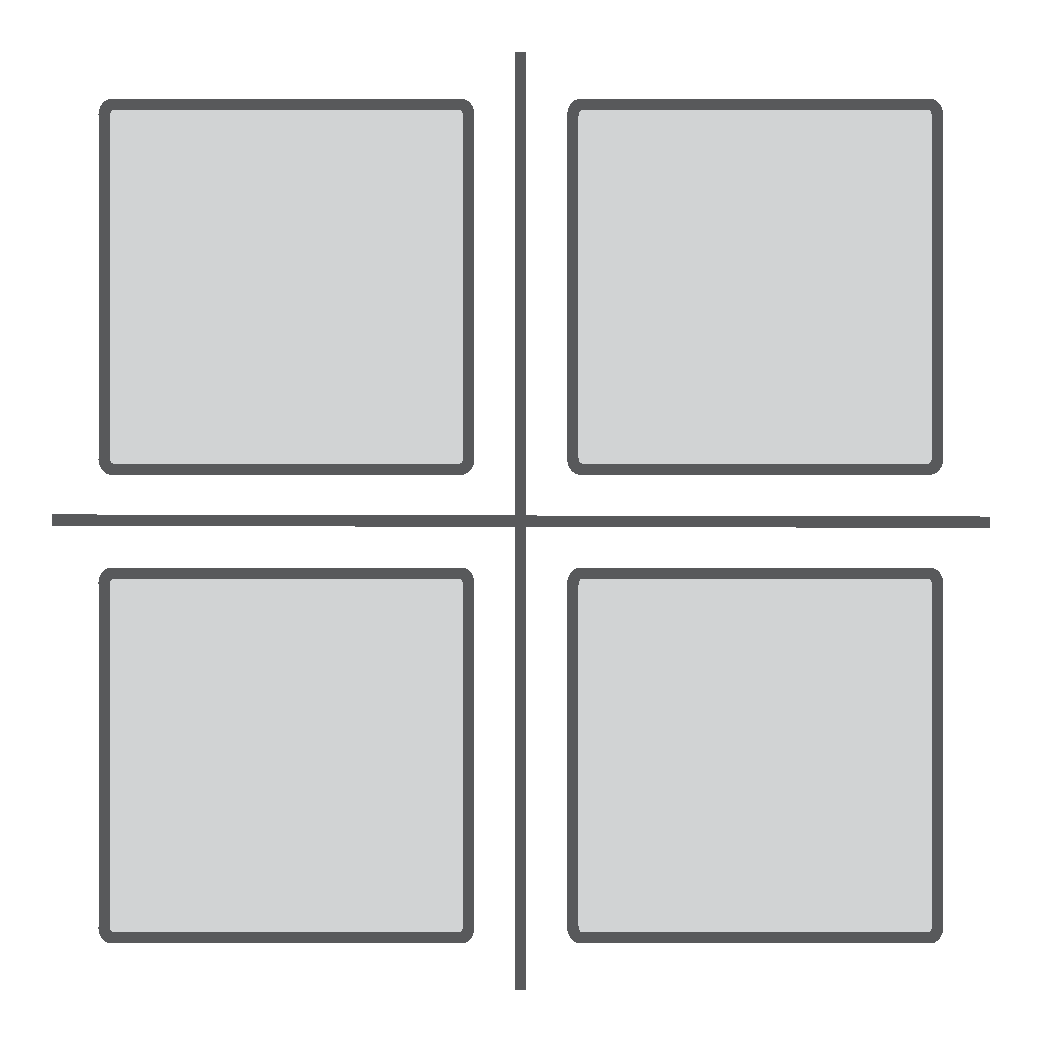
\includegraphics[width=0.3\textwidth]{algorithm-boxes-4}
  }
  \subfigure[5 elements]{
    \label{fig:algorithm-boxes-5}
    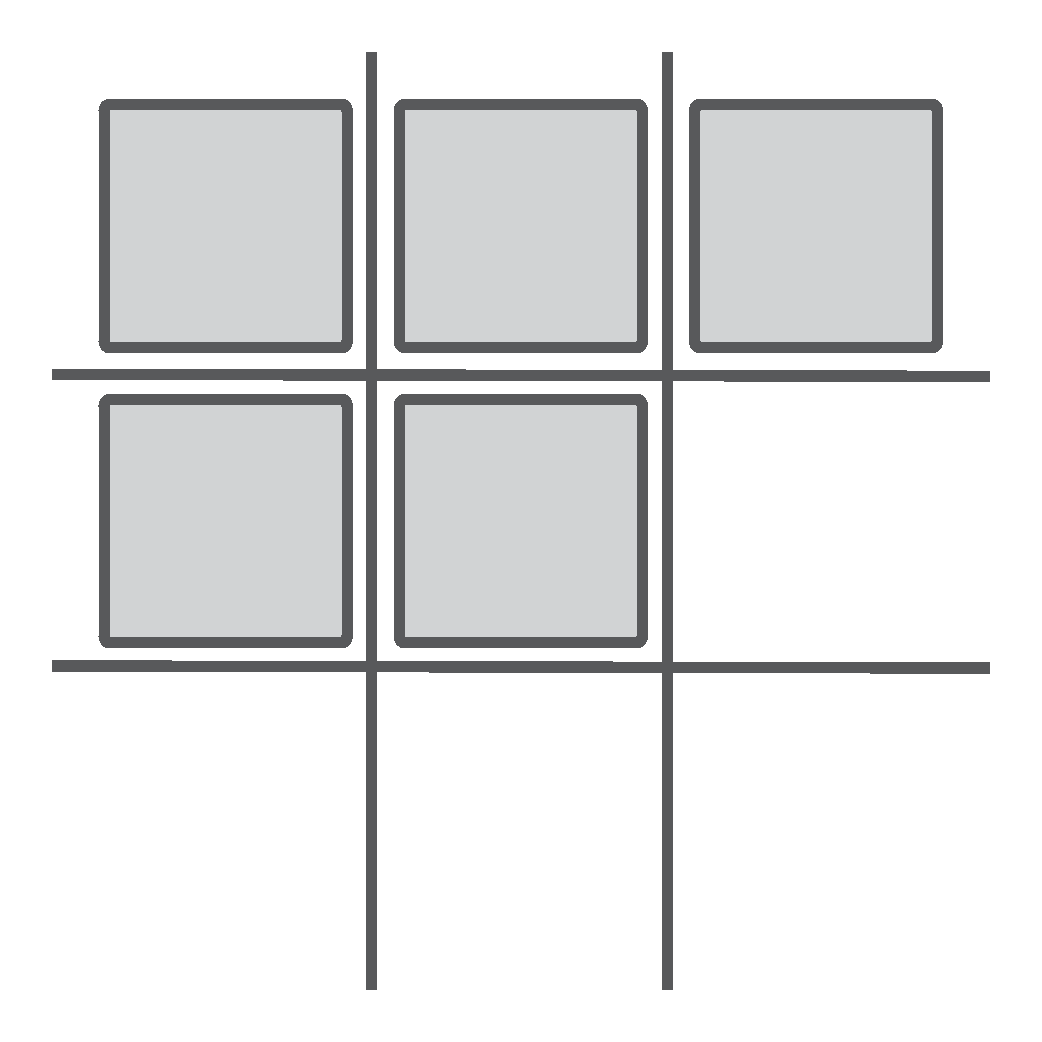
\includegraphics[width=0.3\textwidth]{algorithm-boxes-5}
  }
  \subfigure[6 elements]{
    \label{fig:algorithm-boxes-6}
    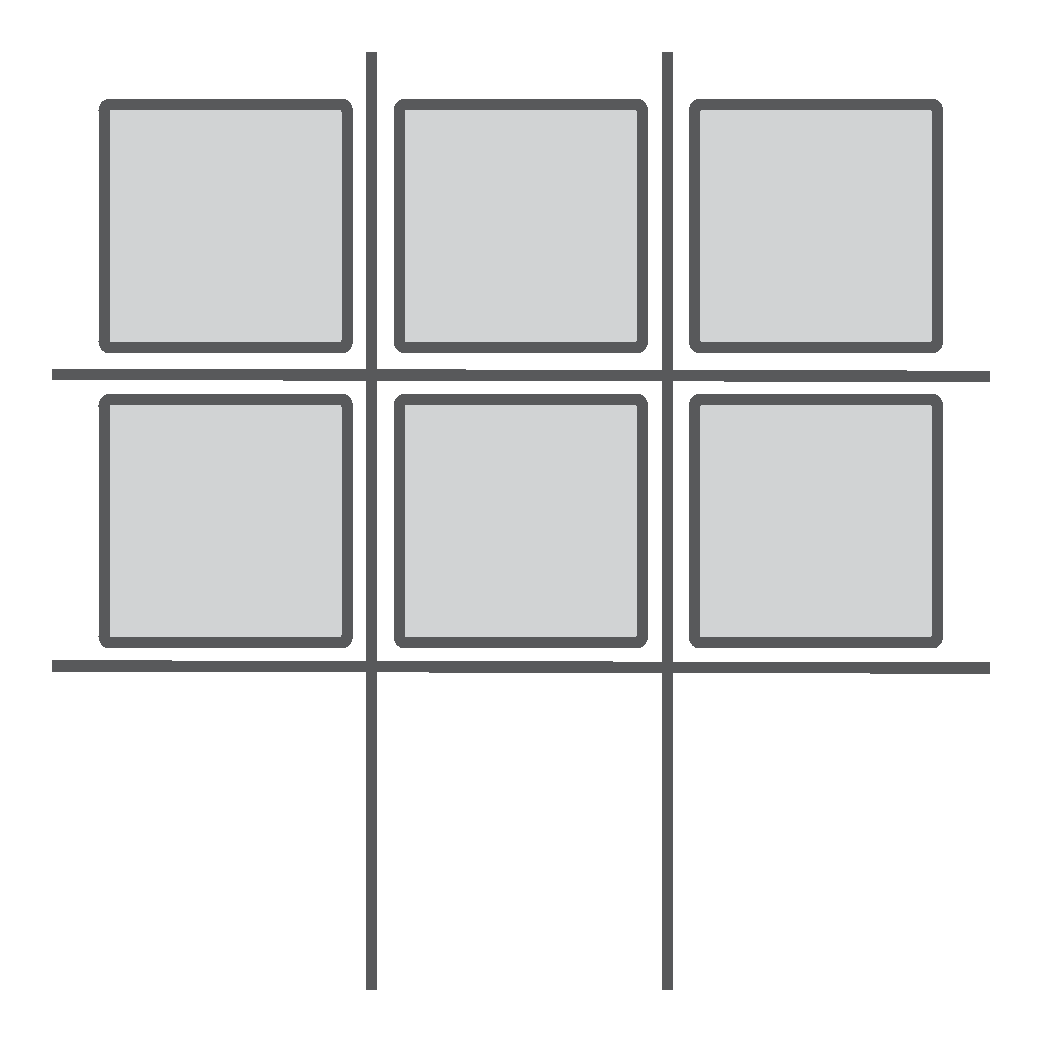
\includegraphics[width=0.3\textwidth]{algorithm-boxes-6}
  }
  \subfigure[7 elements]{
    \label{fig:algorithm-boxes-7}
    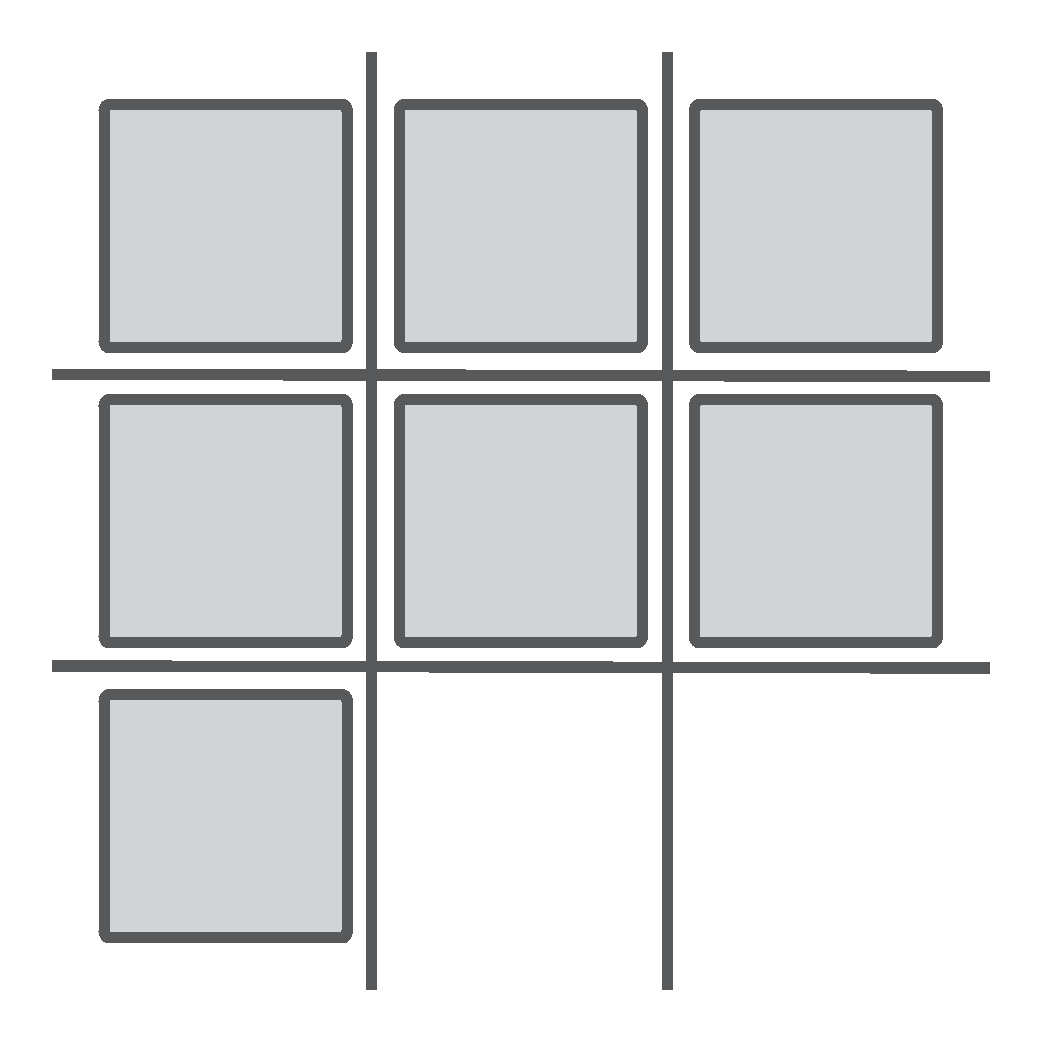
\includegraphics[width=0.3\textwidth]{algorithm-boxes-7}
  }
  \subfigure[8 elements]{
    \label{fig:algorithm-boxes-8}
    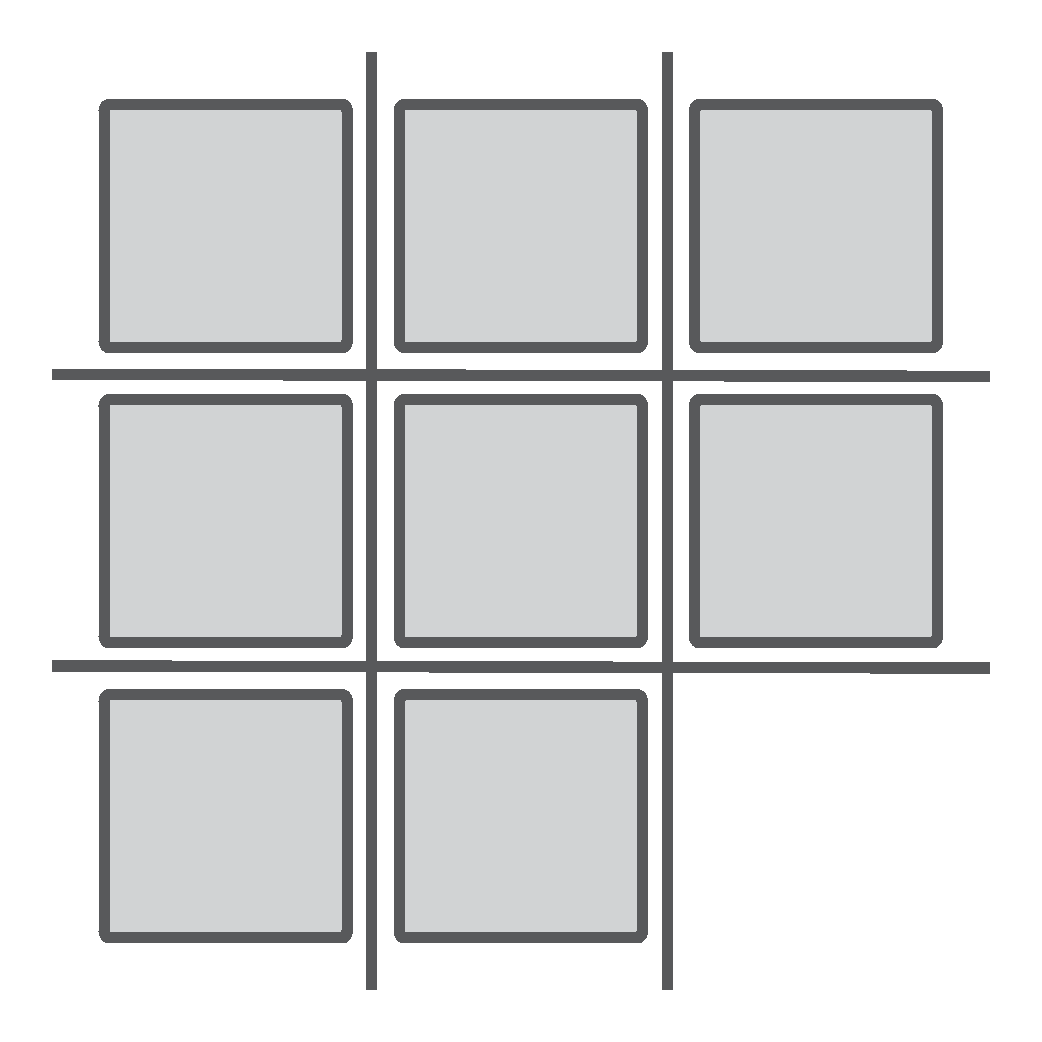
\includegraphics[width=0.3\textwidth]{algorithm-boxes-8}
  }
  \subfigure[9 elements]{
    \label{fig:algorithm-boxes-9}
    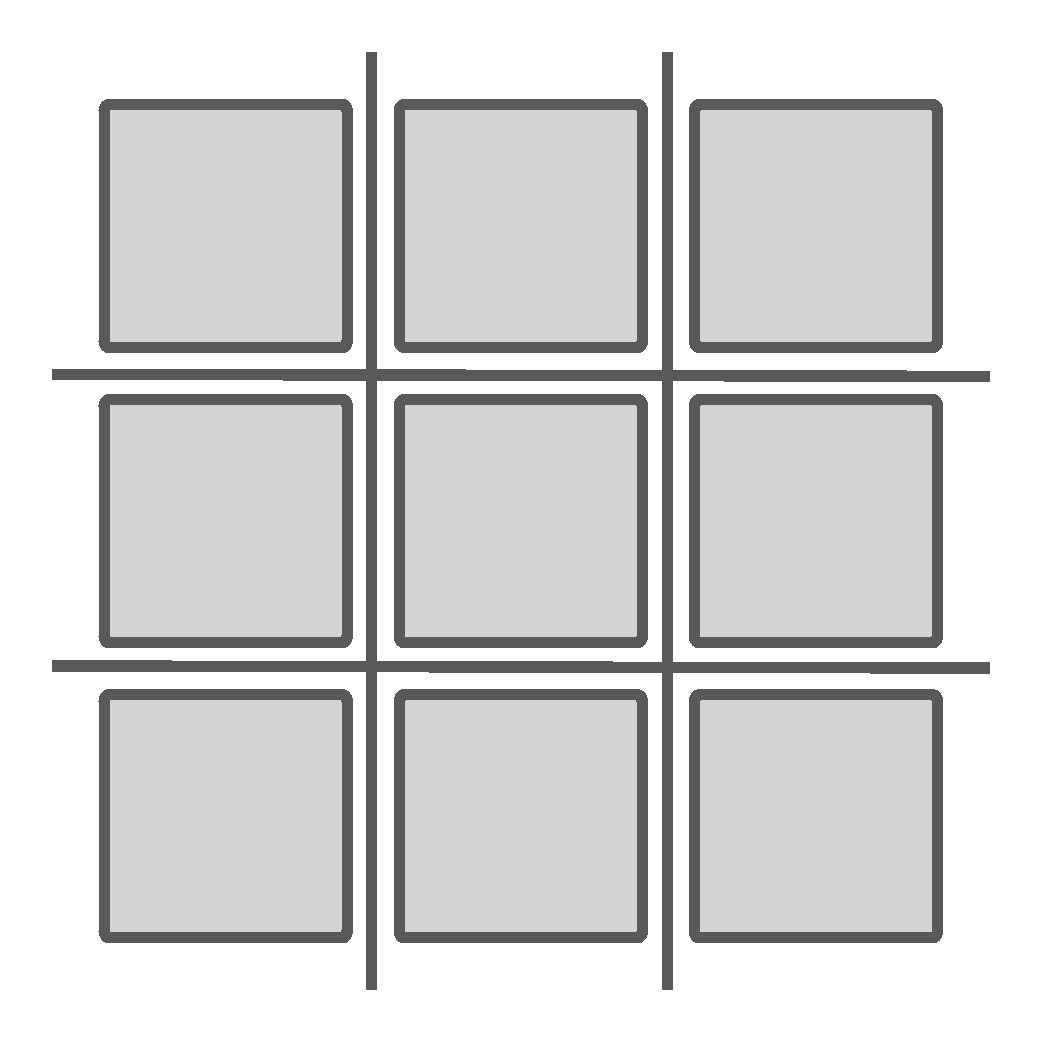
\includegraphics[width=0.3\textwidth]{algorithm-boxes-9}
  }
  \subfigure[11 elements]{
    \label{fig:algorithm-boxes-11}
    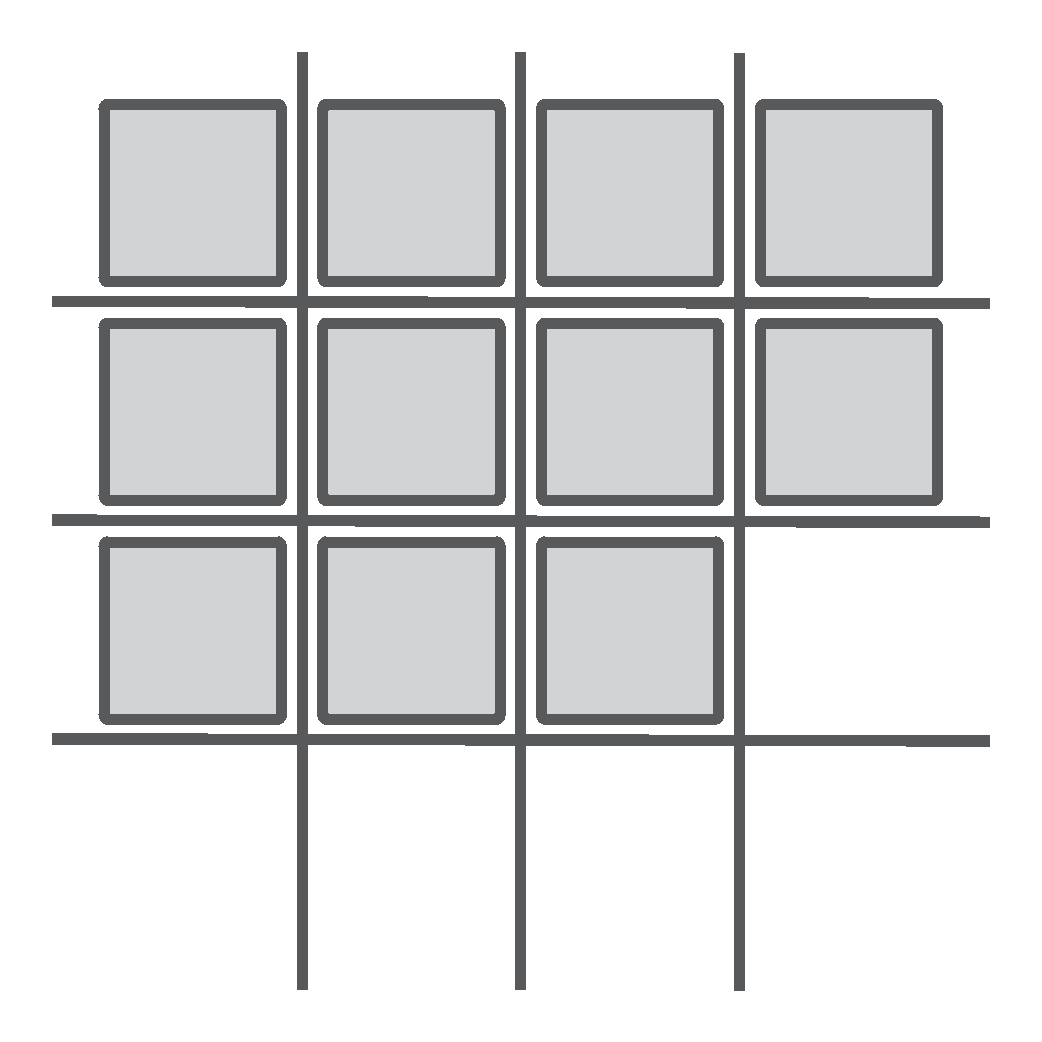
\includegraphics[width=0.3\textwidth]{algorithm-boxes-11}
  }
  \subfigure[12 elements]{
    \label{fig:algorithm-boxes-12}
    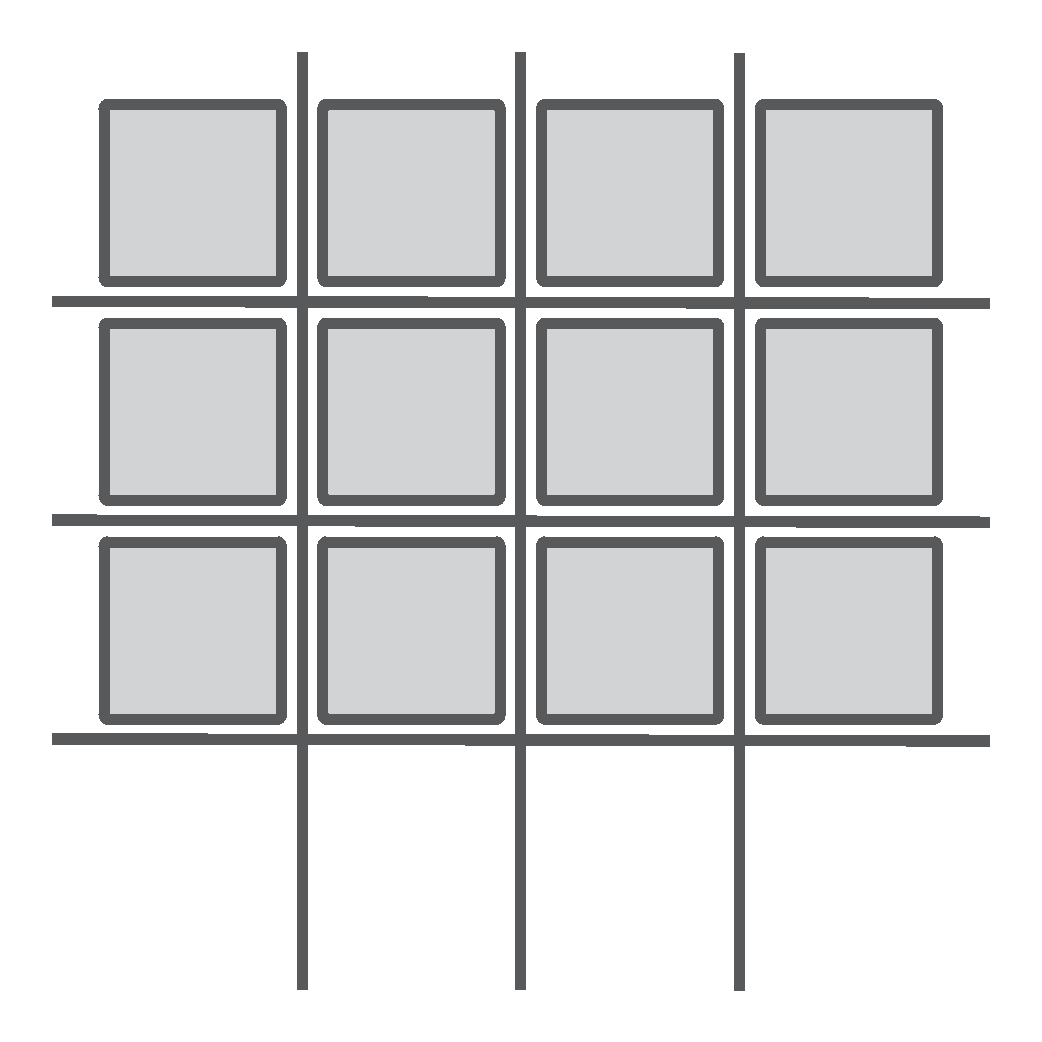
\includegraphics[width=0.3\textwidth]{algorithm-boxes-12}
  }
  \subfigure[13 elements]{
    \label{fig:algorithm-boxes-13}
    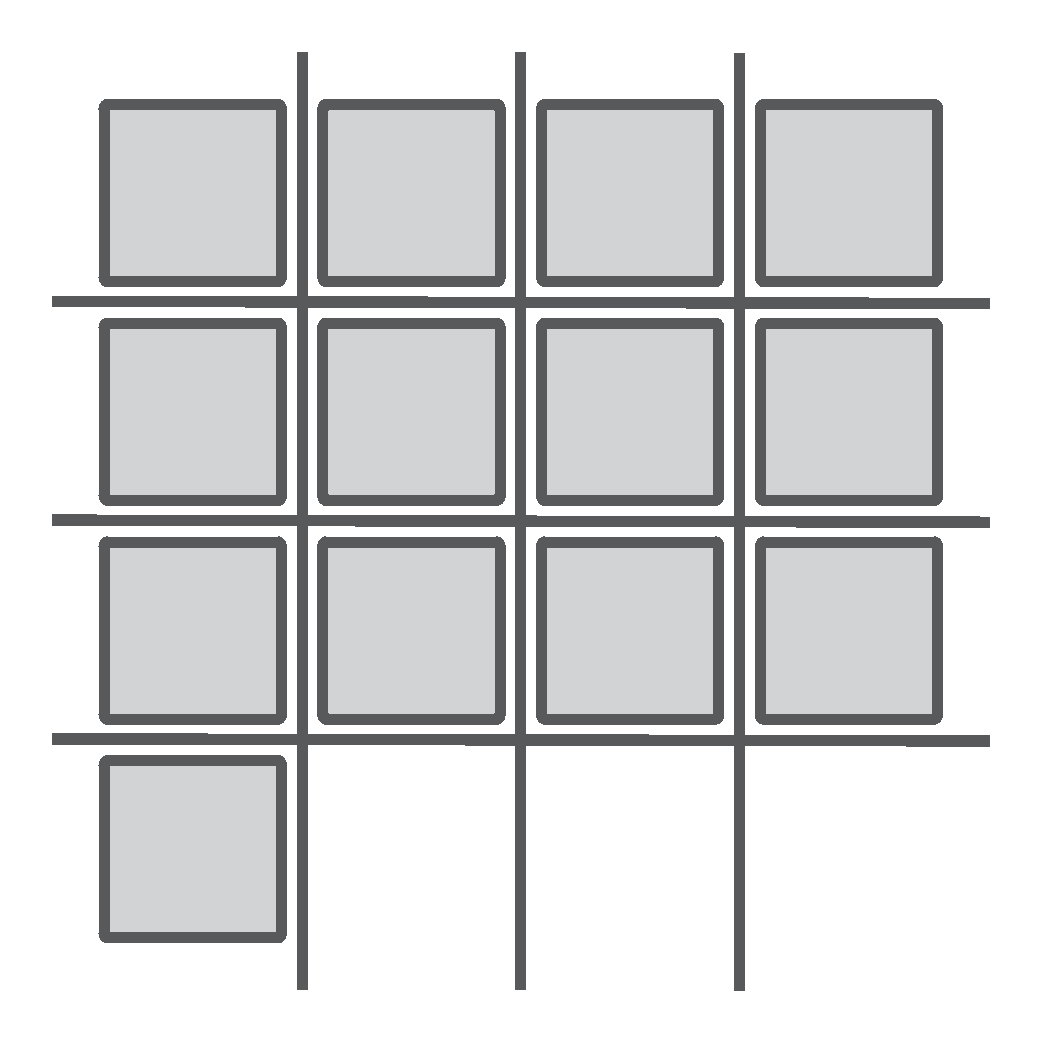
\includegraphics[width=0.3\textwidth]{algorithm-boxes-13}
  }
  \caption{Initial algorithm for positioning devices}
  \label{fig:algorithm-boxes}
\end{figure}

It is easy to see that, at certain points, a whole row of the grid is completely empty, so we are wasting vertical space.
In theory, we could detect when this happens and try to reduce the vertical height of the grid by one, effectively converting this squared grid into a rectangle grid with different number of columns and rows.

Parting from an example: if we have $N = 19$, then we obtain $x = 5$ by applying the previous formula.
This will lead us to a 5x5 grid, but the last row will be completely empty. The question that we have to ask ourselves is:
how big has to be the rectangle grid in order to be able to place this number of elements?

Briefly, the answer is $x \cdot (x - 1)$.
That is a very simple mathematical way of describing that we are decreasing the number of rows by one.
In this case, we need a grid of $5 \times 4$ elements: that will hold up to 20 elements.

To discover whether we have to decrease the number of columns or not, we must compare that number $x \cdot( x - 1)$ with the actual count of elements.
If we know that this number is bigger or equals to the number of elements, then we know that a grid of $x \cdot (x - 1)$ elements can hold those elements.

On the contrary, if we know that this number is strictly lower than the number of elements, then we know that a grid of $x \cdot x$ is unavoidable.
This can be formulated as in eq.~\eqref{gridy}.

\begin{equation}
  Grid_{y} = 
  \begin{cases}
    Grid_{x} - 1 & \text{if } N \leq Grid_{x} \cdot (Grid_{x} - 1),\\
    Grid_{x} & \text{if } N > Grid_{x} \cdot (Grid_{x} - 1).
  \end{cases} \label{gridy}
\end{equation}

Another question appears: Do we need to shrink the grid only by one?
Is there any case in which we have to shrink the grid by two or more?

The answer is no.

Well, in Figure~\vref{fig:algorithm-boxes} is obvious that this does not happen with sixteen elements or less, and that is a sufficiently big number of devices a person can own in the system.
But we can mathematically prove this by calculating if a grid of $(x - 1) \cdot (x - 1)$ elements can hold more elements that the grid of $x \cdot (x - 2)$.

If that is the case, then we would not need to shrink the grid in any case by two because the grid will be already horizontally shorter.
It is quick to prove this is true following the steps explained from eq.~\eqref{xdem1} to eq.~\eqref{xdem3}.

\begin{eqnarray}
  (x-1) \cdot (x-1) &<& x \cdot (x-1) \label{xdem1} \\
  x^2-2x+1 &<& x^2-2x \label{xdem2} \\
  1 &<& 0 \label{xdem3}
\end{eqnarray}

Figure~\vref{fig:algorithm-boxes-fixed} shows the results after applying this final algorithm, filling more space in some situations.
Using this algorithm we can calculate the height, width, vertical and horizontal offset for every element, so that it keeps its aspect ratio while placing it in the middle of the allocated space.

\begin{figure}[htbp]
  \centering
  \subfigure[1 element]{
    \label{fig:algorithm-boxes-1-fixed}
    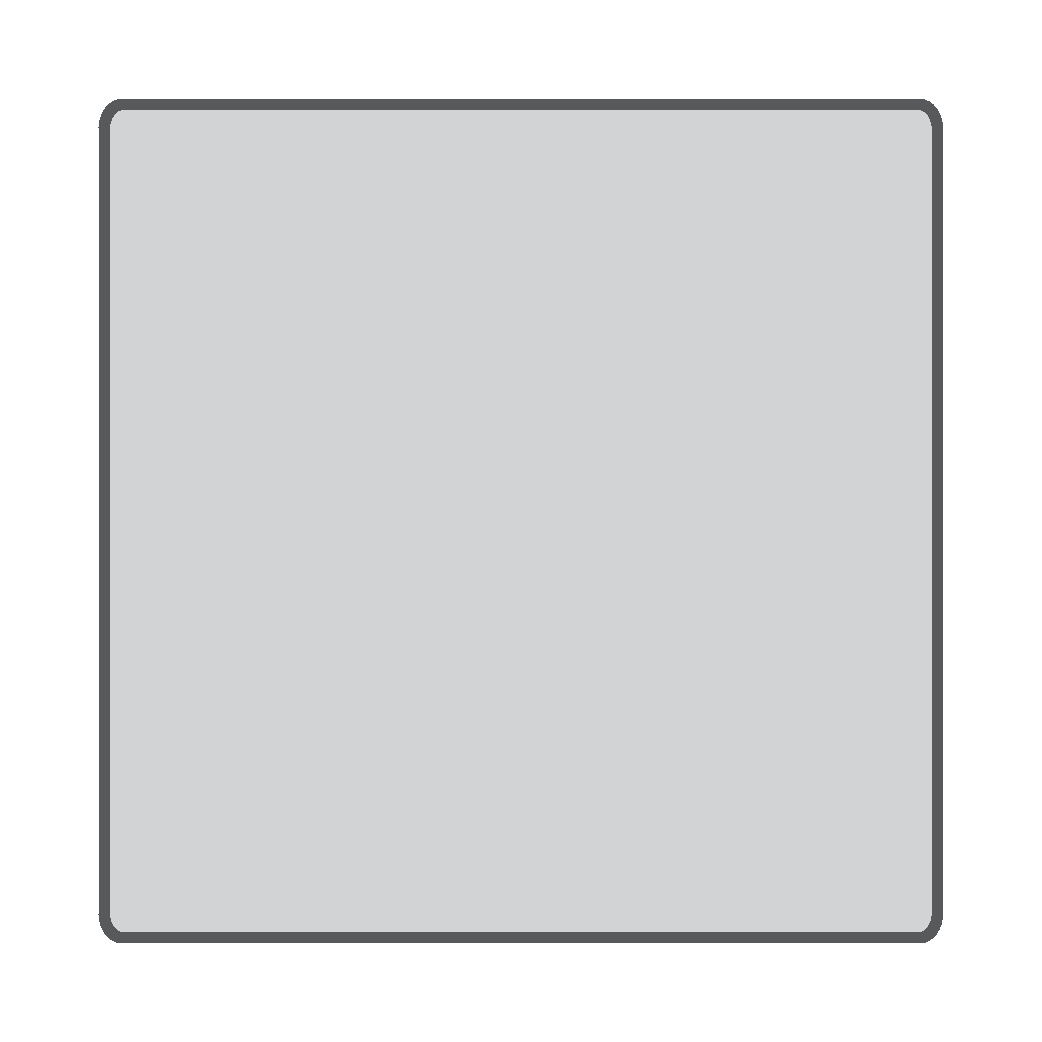
\includegraphics[width=0.3\textwidth]{algorithm-boxes-1}
  }
  \subfigure[2 elements]{
    \label{fig:algorithm-boxes-2-fixed}
    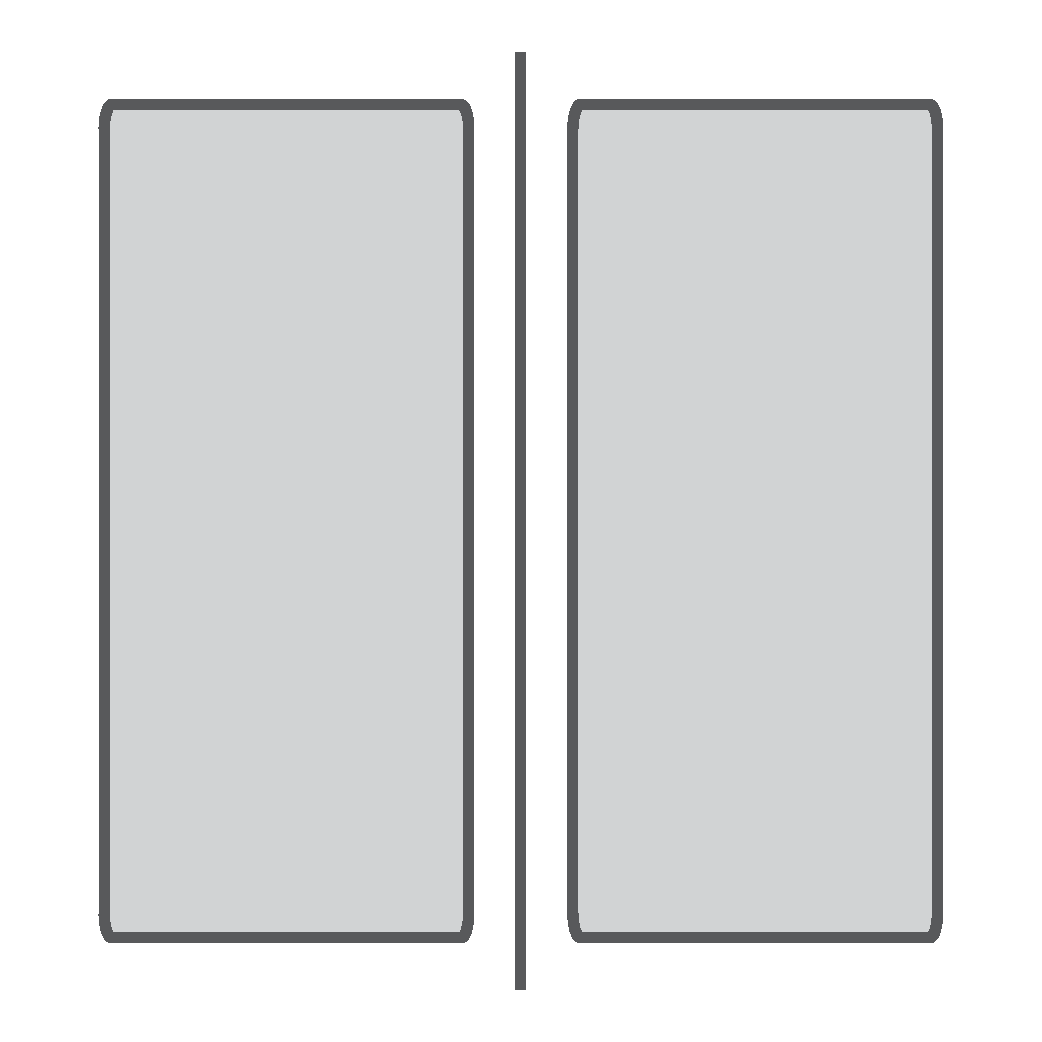
\includegraphics[width=0.3\textwidth]{algorithm-boxes-2-fixed}
  }
  \subfigure[3 elements]{
    \label{fig:algorithm-boxes-3-fixed}
    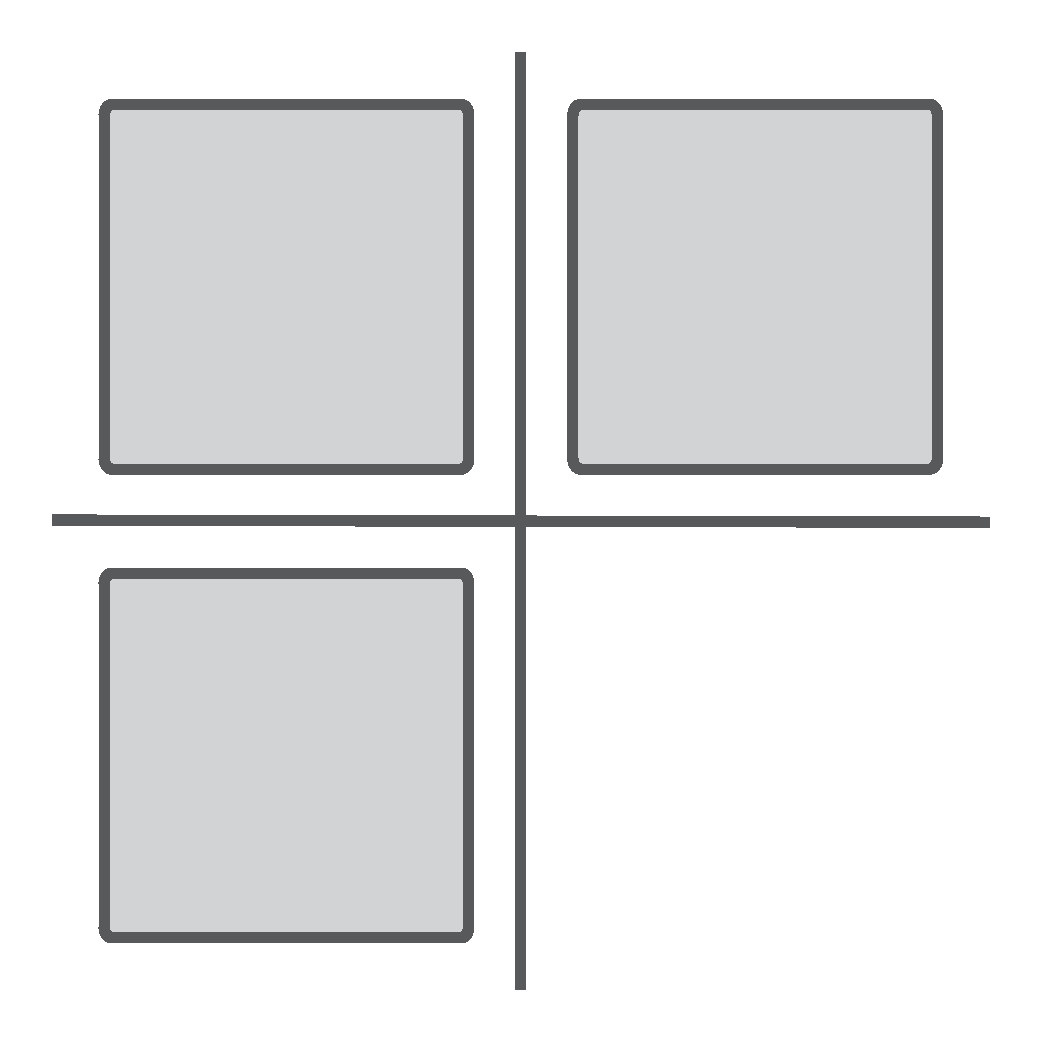
\includegraphics[width=0.3\textwidth]{algorithm-boxes-3}
  }
  \subfigure[4 elements]{
    \label{fig:algorithm-boxes-4-fixed}
    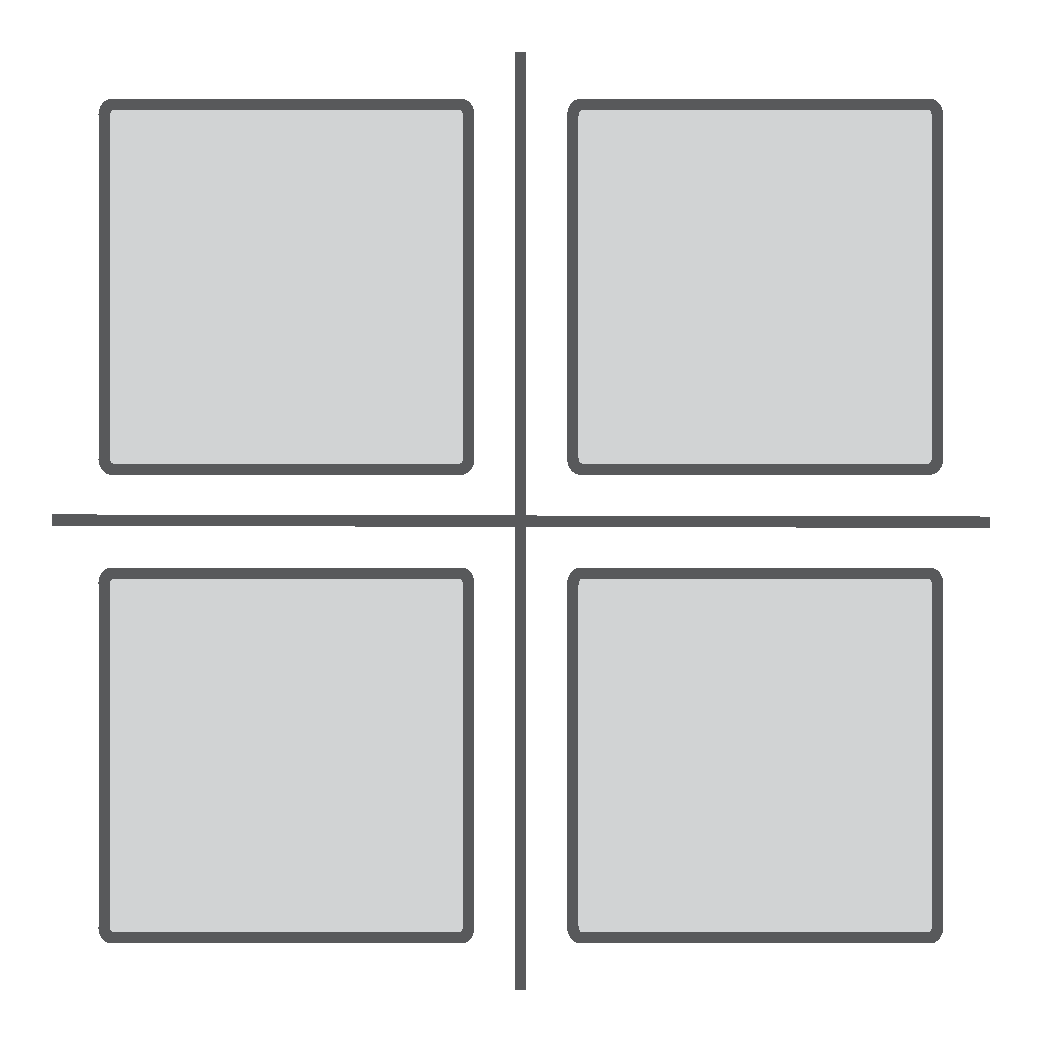
\includegraphics[width=0.3\textwidth]{algorithm-boxes-4}
  }
  \subfigure[5 elements]{
    \label{fig:algorithm-boxes-5-fixed}
    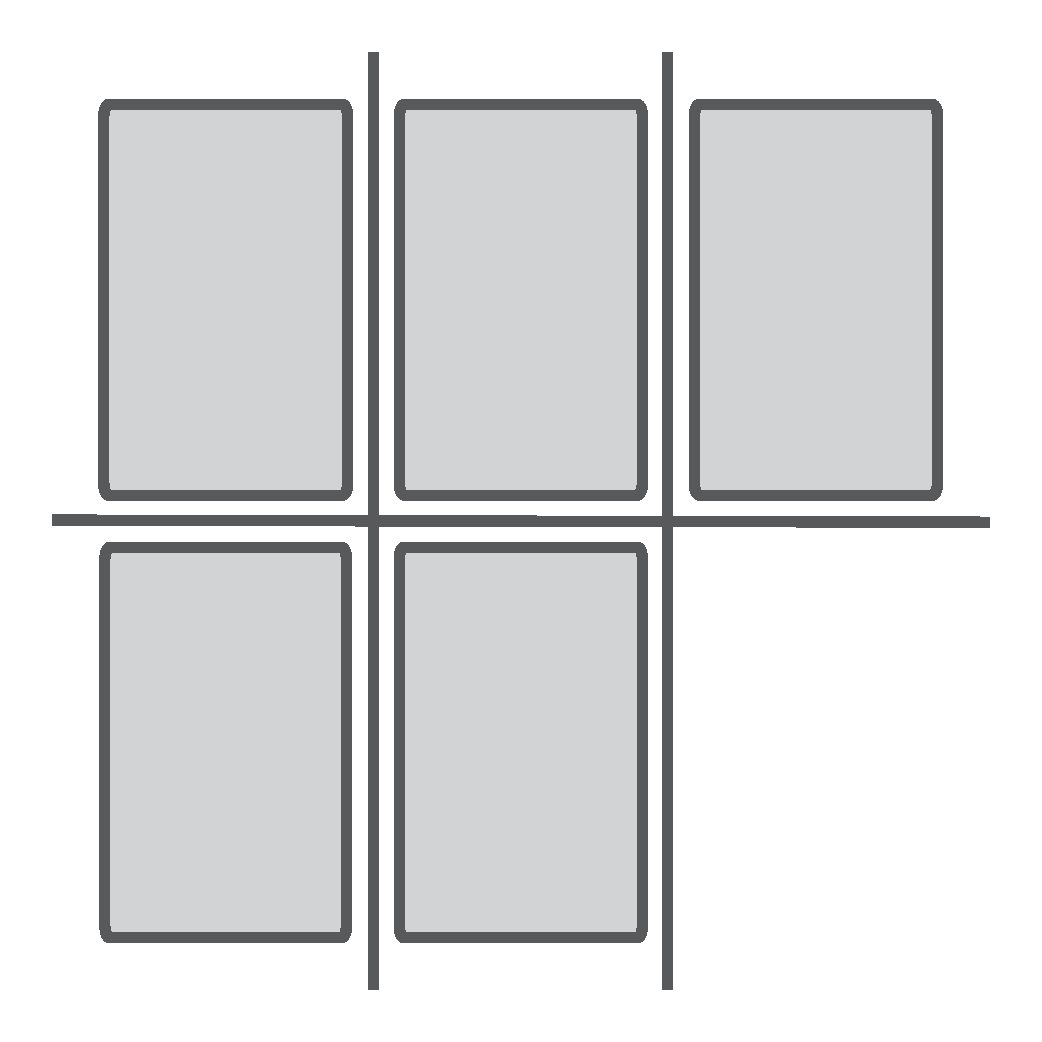
\includegraphics[width=0.3\textwidth]{algorithm-boxes-5-fixed}
  }
  \subfigure[6 elements]{
    \label{fig:algorithm-boxes-6-fixed}
    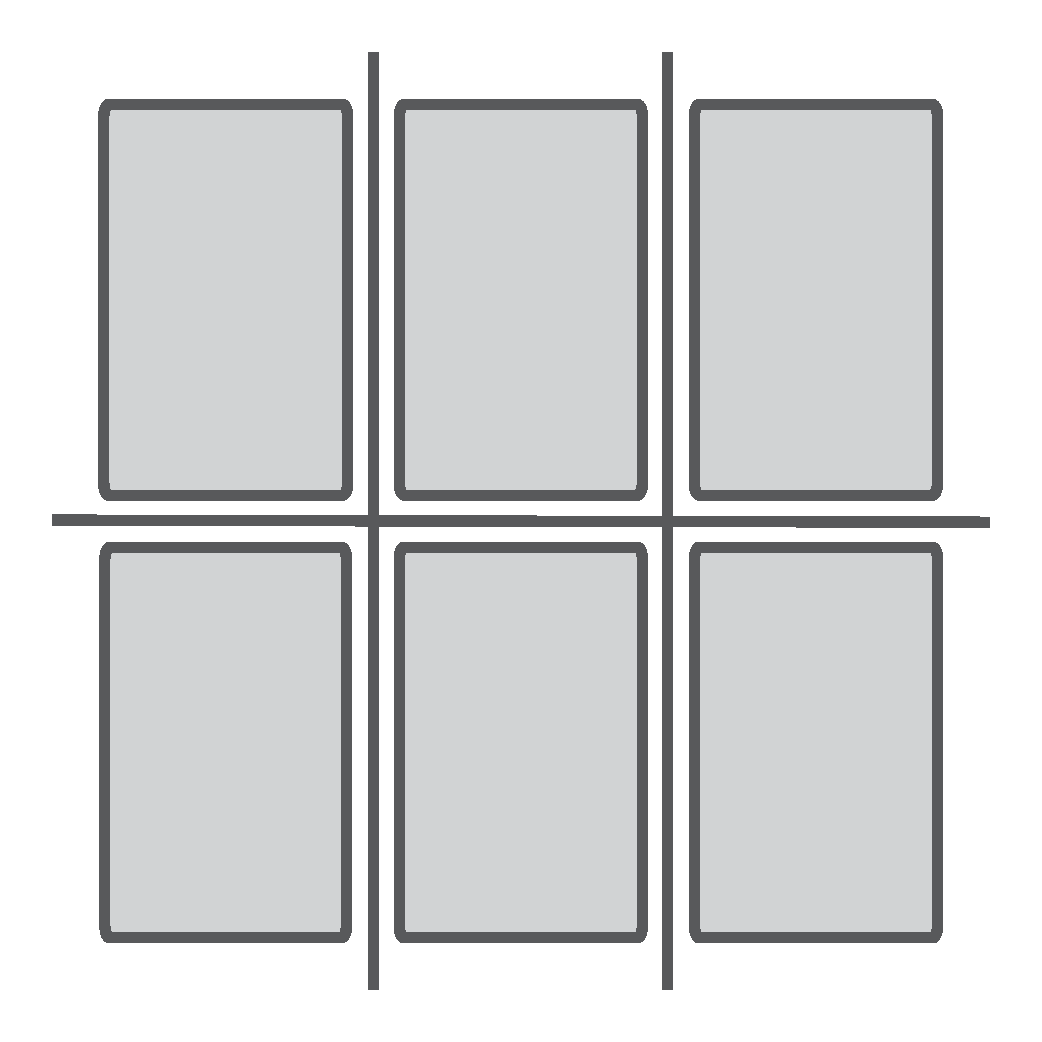
\includegraphics[width=0.3\textwidth]{algorithm-boxes-6-fixed}
  }
  \subfigure[7 elements]{
    \label{fig:algorithm-boxes-7-fixed}
    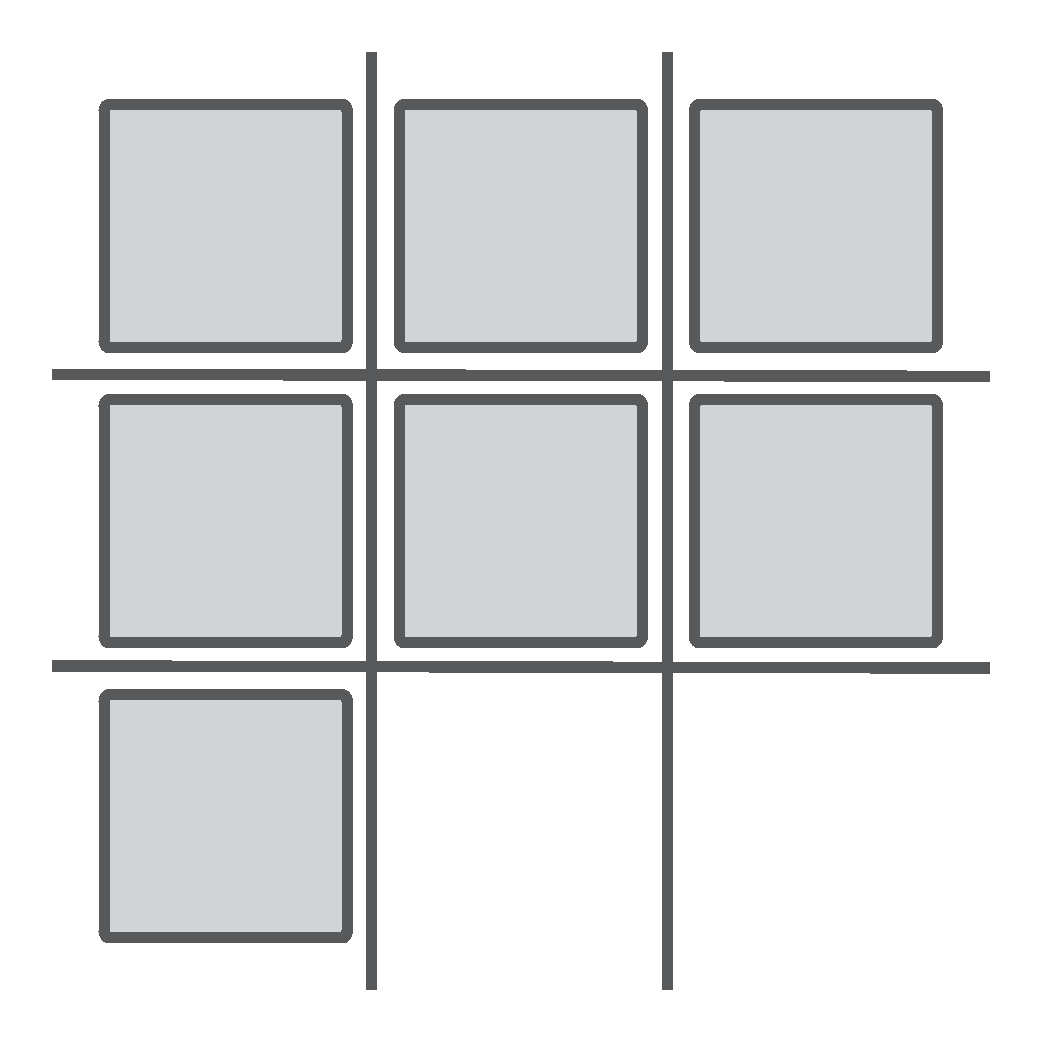
\includegraphics[width=0.3\textwidth]{algorithm-boxes-7}
  }
  \subfigure[8 elements]{
    \label{fig:algorithm-boxes-8-fixed}
    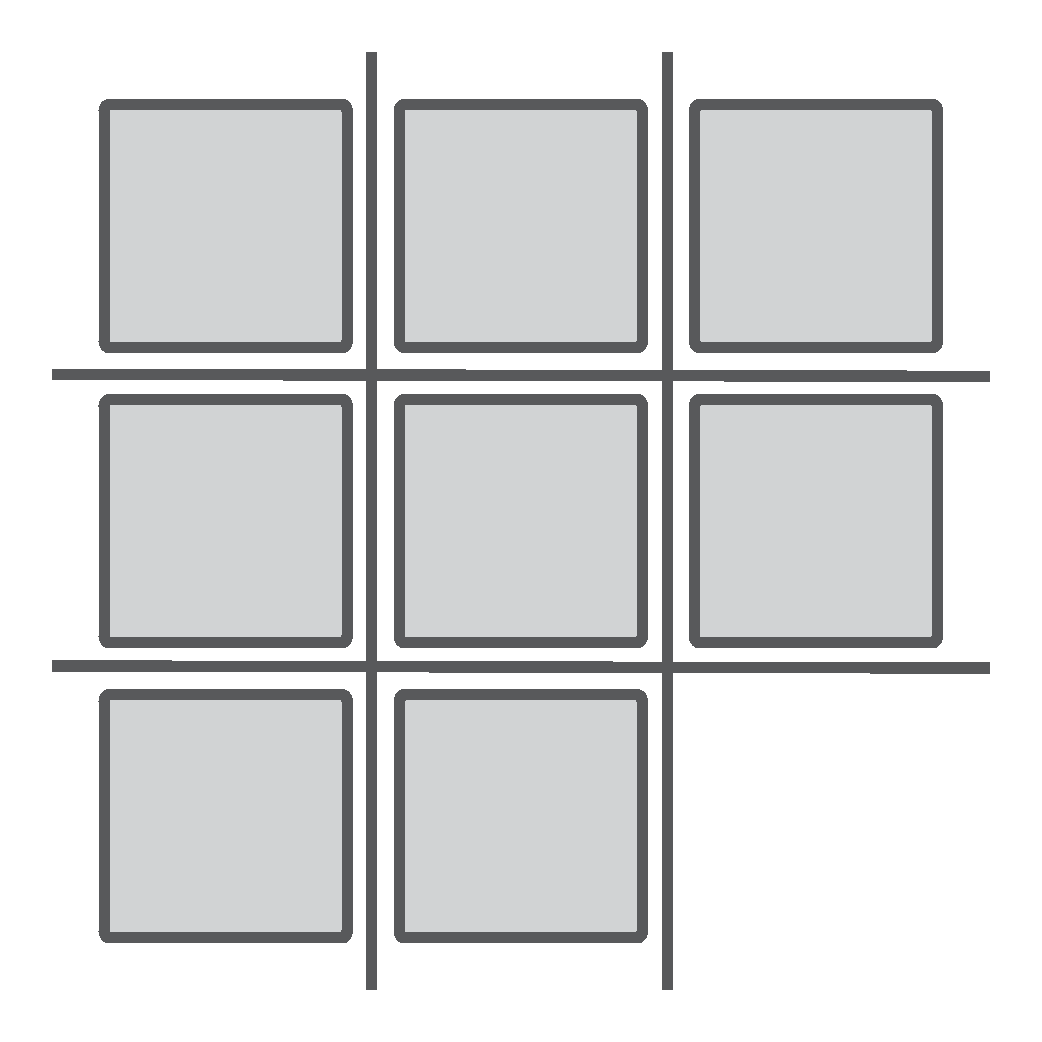
\includegraphics[width=0.3\textwidth]{algorithm-boxes-8}
  }
  \subfigure[9 elements]{
    \label{fig:algorithm-boxes-9-fixed}
    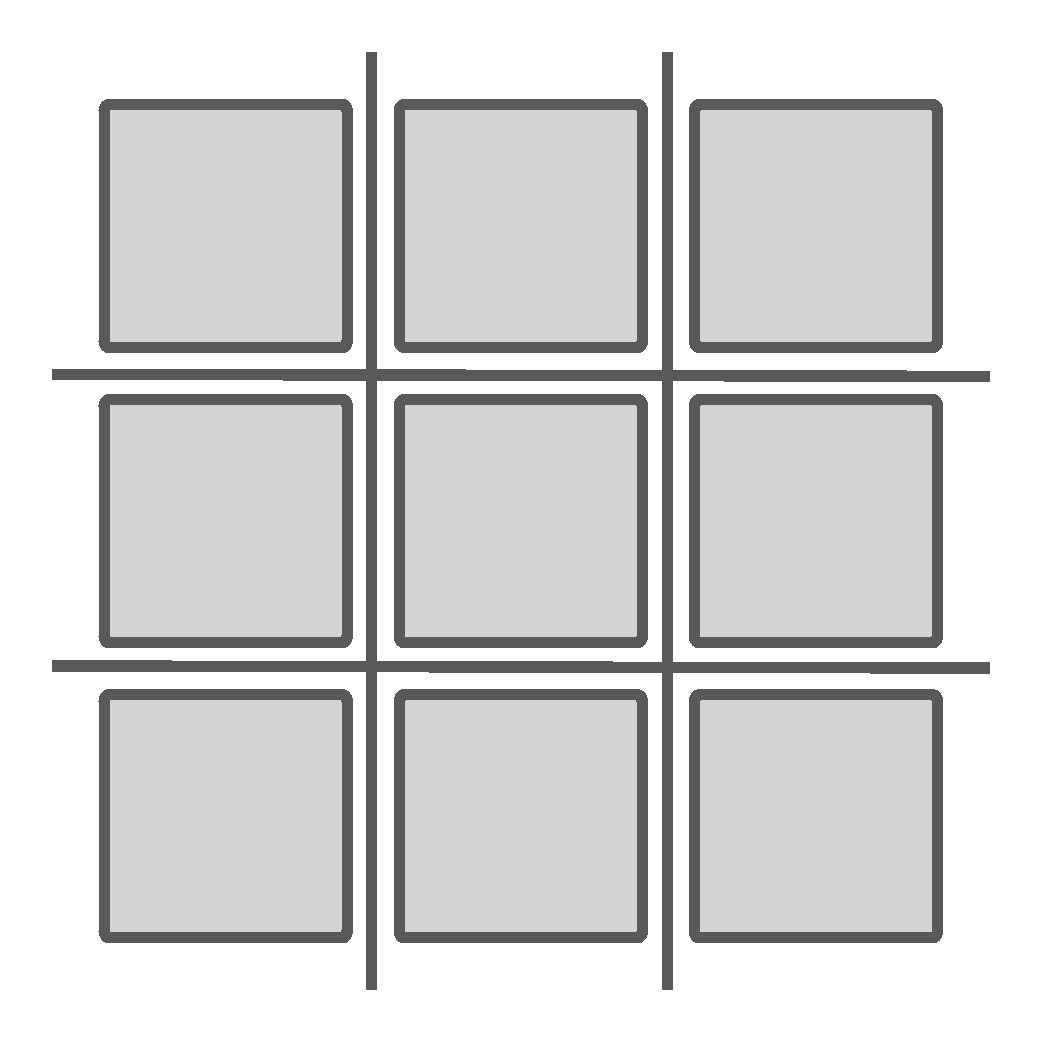
\includegraphics[width=0.3\textwidth]{algorithm-boxes-9}
  }
  \subfigure[11 elements]{
    \label{fig:algorithm-boxes-11-fixed}
    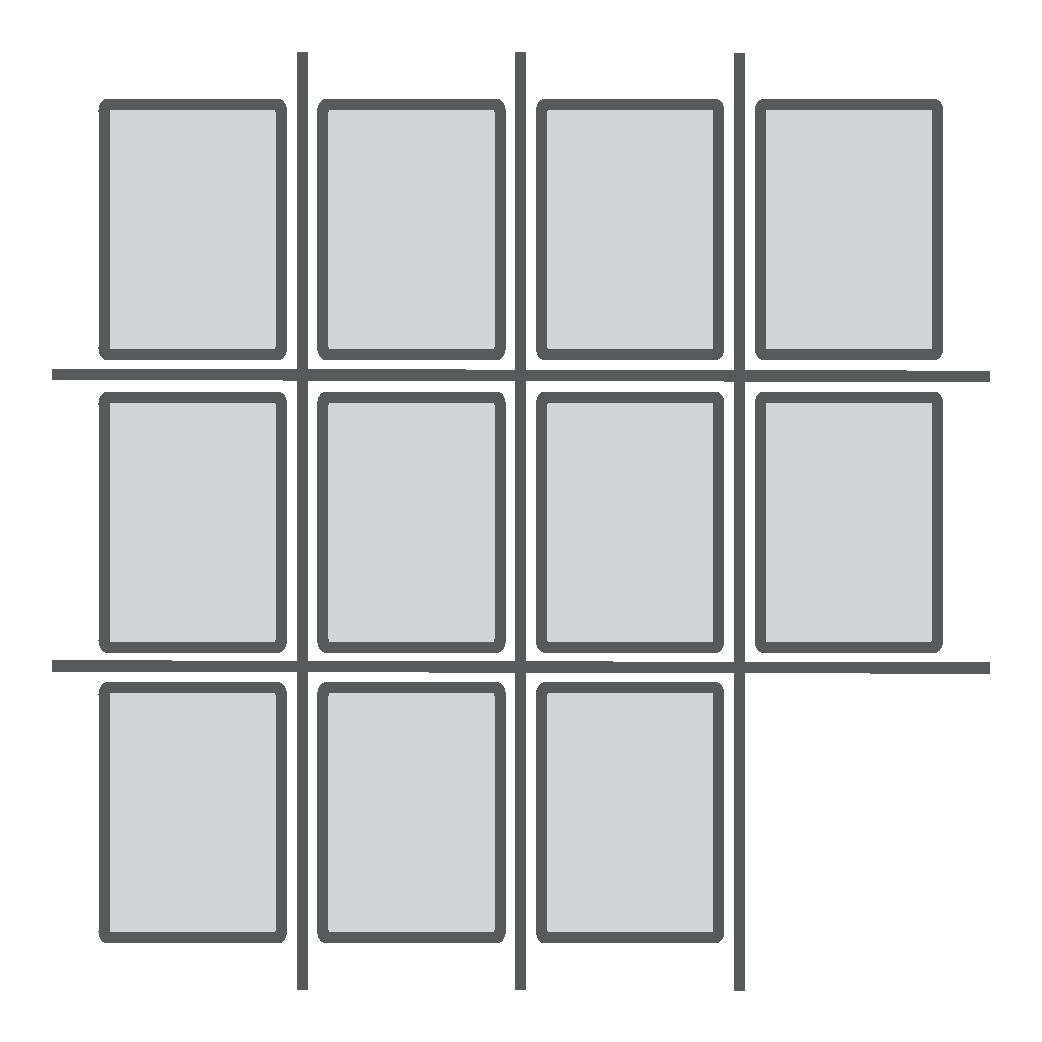
\includegraphics[width=0.3\textwidth]{algorithm-boxes-11-fixed}
  }
  \subfigure[12 elements]{
    \label{fig:algorithm-boxes-12-fixed}
    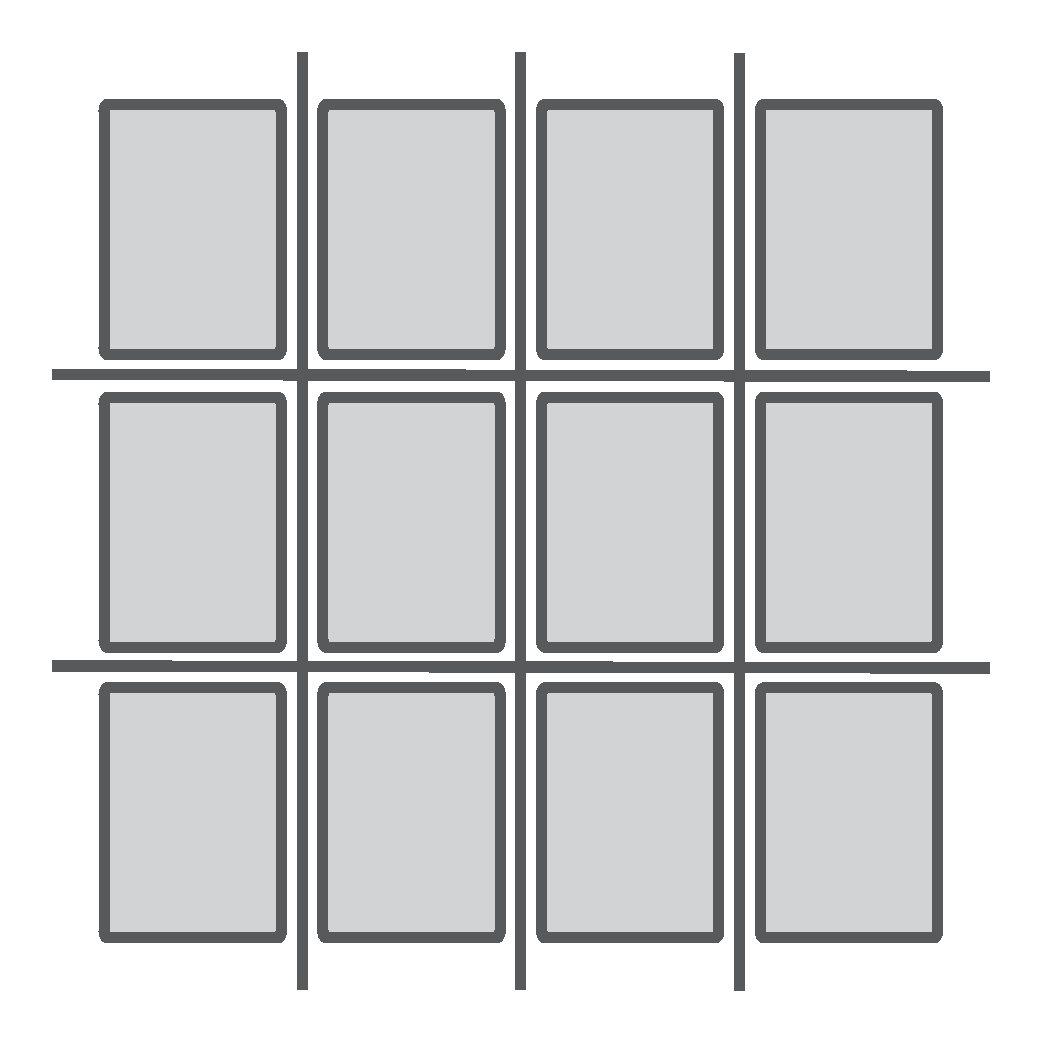
\includegraphics[width=0.3\textwidth]{algorithm-boxes-12-fixed}
  }
  \subfigure[13 elements]{
    \label{fig:algorithm-boxes-13-fixed}
    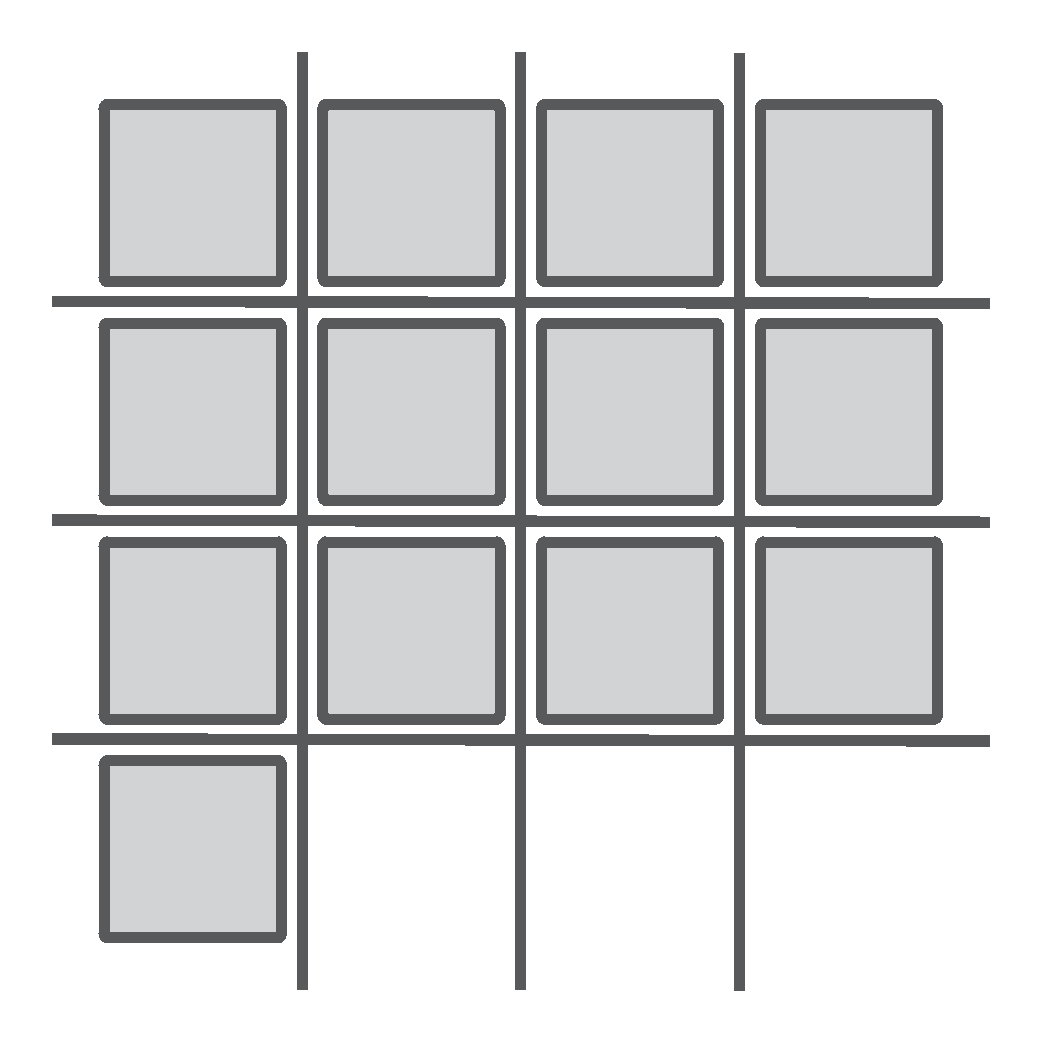
\includegraphics[width=0.3\textwidth]{algorithm-boxes-13}
  }
  \caption{Final algorithm for positioning devices}
  \label{fig:algorithm-boxes-fixed}
\end{figure}

If we want to work with percentages, we only have to divide the size of the container between the number of columns and rows.
For example, if we want to fill the container at 100\%, then every element will be of size $100/x \times 100/y$.
The actual values for the offset needed for every particular element is then easy to calculate if we fill the canvas one by one.

% subsection algorithm (end)

\subsection{Remembering Positions} % (fold)
\label{sub:remembering_positions}

Next time a user visits this page, the system will remember the last position of those elements instead of calculating the grid again.
Because the user can change the size of the window at any time, we cannot relay on fixed positioning with pixels, because our canvas could be bigger or, worse, smaller than the one we have calculated.
Besides being not very elegant, we can find several situations where the page is unusable.

The best way to avoid all that trouble is treating every position or size in terms of percentages.
This is how is done in the code, and it allows the user to resize the window at any time: the devices will be resized dinamically according to that window size.

To store and retrieve painlessly these values, we are going to take advantage of a useful \idx{MooTools} class: \idc{Hash.Cookie} \cite{MooHashCookie}.
With this utility, we only have to specify the name for the \idc{Cookie} and we can store a \idc{Hash} into a \idc{Cookie} without worrying about the \idc{Cookie} itself.
Besides loading the data of the \idc{Cookie} directly on the \idc{Hash} at its creation, if we change a value of the \idc{Hash} it will be automatically updated in the \idc{Cookie}.

The reason for using a \idc{Cookie} is mostly because it reduces complexity on the server, since it does not have to store the position of every device.
Other good reason is that it is the most simple way of allowing different arrangements in different places; for example the user may want to arrange radically different its devices in a big screen like in a TV or on a smaller screen like in a netbook.
Finally, it is universal as it is supported by almost every browser.

The final decision is to have one \idc{Cookie} for each device.
This is very straightforward for the implementation, since a \idc{Cookie} can
have the name of the container.
Each \idc{Hash} that is stored in every \idc{Cookie} is composed by the four
values needed for positioning the element: \idc{offsetX}, \idc{offsetY},
\idc{width} and \idc{height}.
These values are percentages respect the container (the devices list) and a
\idc{Hash} example is presented in Listing~\vref{cookiehash}.

\begin{lstlisting}[language=JavaScript,label=cookiehash,caption=Cookie Hash example]
  {
    offsetX: 15,
    offsetY: 50,
    height: 10,
    width: 20
  }
\end{lstlisting}

Then, each time the object size or dimension changes, the \idc{Hash} (and therefore the \idc{Cookie}) is updated.
These changes happen mostly in two situations: when we resize a device (changing its size but no its position) or when we move around a device (changing its position but not its size).
% subsection remembering_positions (end)
% section positioning (end)